\onehalfspaced

\section{Choosing Better Translators}

The second mechanism that we use to optimize cost is to reduce the number of non-professional translators that we hire.  Our goal is to quickly identify whether Turkers are good or bad translators, so that we can continue to hire only the good translators and stop hiring the bad translators after they are identified as such. 
%
Before presenting our method, we first demonstrate that Turkers produce consistent quality translations over time.


\subsection{Turkers' behavior in translating sentences}

Do Turkers produce good (or bad) translations consistently or not? Are some Turkers  consistent and others not? We used the professional translations as a gold-standard to analyze the individual Turkers, and we found that most Turkers' performance stayed surprisingly consistent over time. 

Figure \ref{fworkerperf} illustrates the consistency of workers' quality by plotting quality of their individual translations on a timeline. The translation quality is computed based on the BLEU against professional translations. Each tick represent a single translation and depicts the BLEU score using two colors. The tick is black if its BLEU score is higher than the median and it is light grey otherwise. Good translators tend to produce consistently good translations and bad workers rarely produce good translations.





 \begin{figure*}[!ht]
\centering
\begin{minipage}[t]{.475\textwidth}
 \centering
  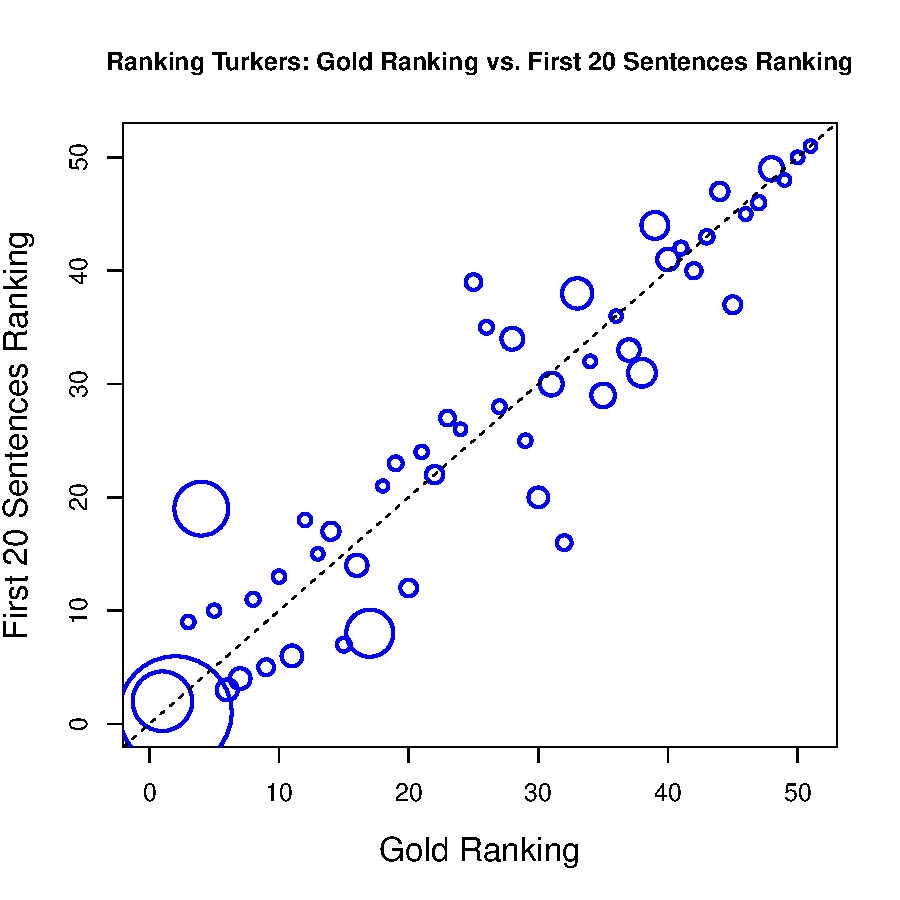
\includegraphics[width=2.8in]{AllFeatureWithCali/2hitranking.pdf}
   \caption{Correlation between gold standard ranking and ranking computed using the first 20 sentences as calibration. Each bubble represents a worker. The radius of each bubble shows the relative volume of translations completed by the worker. 
The  weighted correlation is 0.94.  }
\label{first2hitrank}
\end{minipage}
\hfill
\begin{minipage}[t]{.475\textwidth}
  \centering
  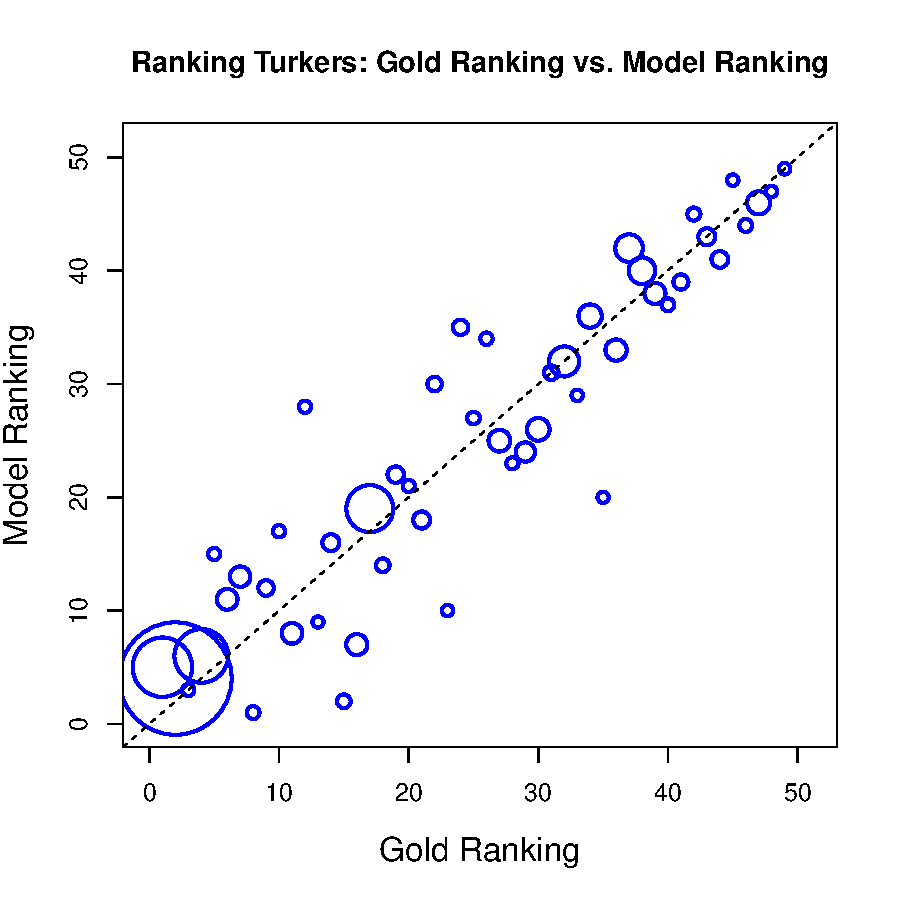
\includegraphics[width=2.8in]{AllFeatureWithCali/allfeaturelinear.pdf}
  \centering
     \caption{Correlation between gold standard ranking and our model's ranking. 
The corresponding weighted correlation is 0.95.}
  \label{modelrank}
\end{minipage}
\end{figure*}


\begin{comment}
\begin{figure}
  \centering
  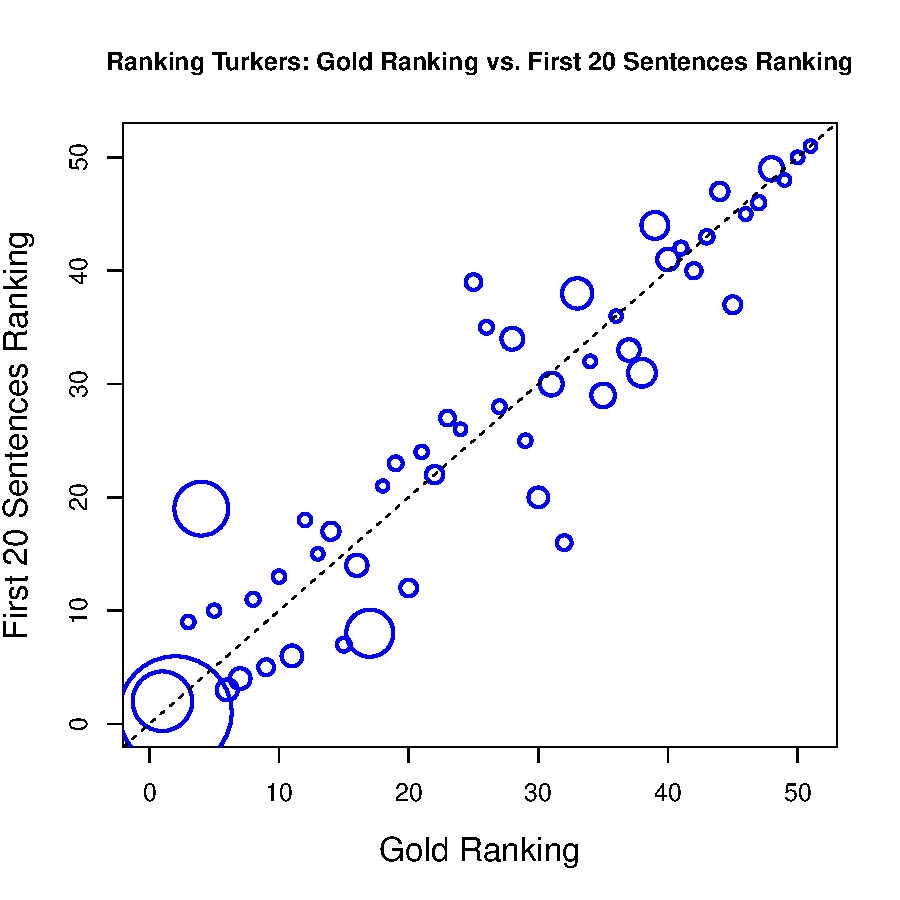
\includegraphics[width=\linewidth]{AllFeatureWithCali/2hitranking.pdf}
  \caption{Correlation between gold standard ranking and ranking computed using the first 20 sentences as calibration. Each bubble represents a worker. The radius of each bubble shows the relative volume of translations completed by the worker. 
The  weighted correlation is 0.94.  }
    \label{first2hitrank}
\end{figure}
%
\begin{figure}
  \centering
  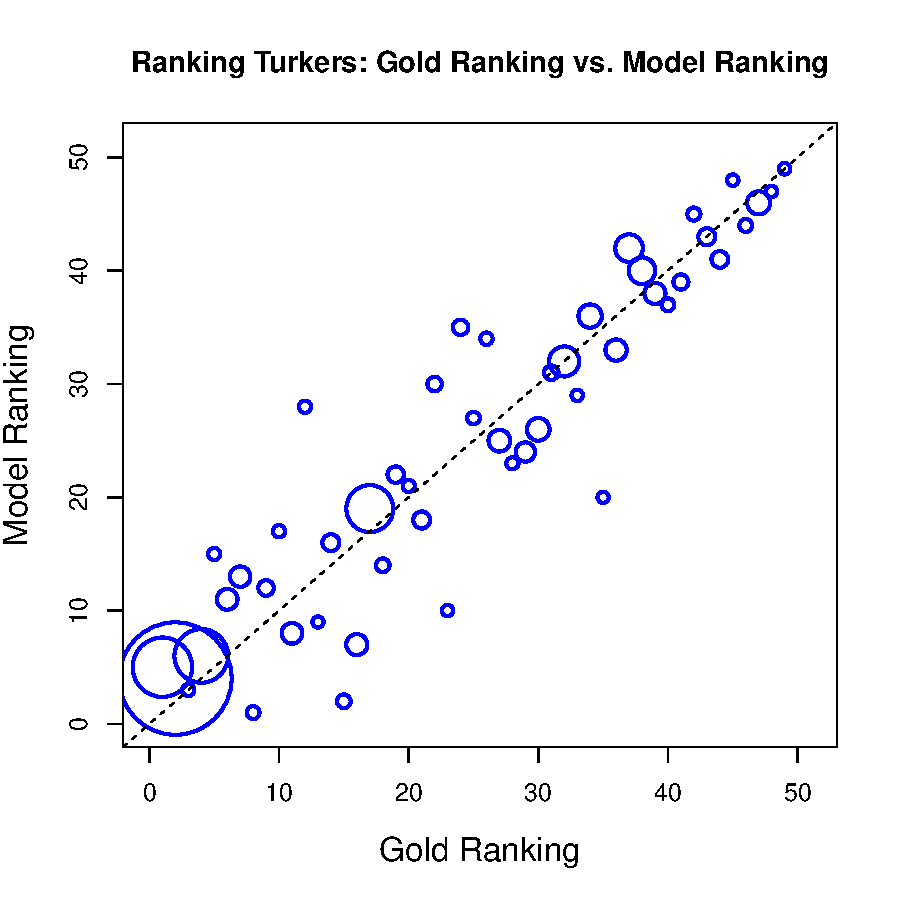
\includegraphics[width=\linewidth]{AllFeatureWithCali/allfeaturelinear.pdf}
  \caption{Correlation between gold standard ranking and our model's ranking. 
The corresponding weighted correlation is 0.95.}
    \label{modelrank}
\end{figure}
\end{comment}


\subsection{Evaluating Rankings}
We use weighted Pearson correlation \cite{pozzi2012exponential} to evaluate our ranking of workers against gold standard ranking. Since workers translated different number of sentences, it is more important to rank the workers who translated more sentences correctly. Taking the importance of workers into consideration, we set a weight to each worker using the number of translations he or she submitted when calculating the correlation.
Given two lists of worker scores \textit{x} and \textit{y} and the weight vector \textit{w}, the weighted Pearson correlation $\rho$ can be calculated as:
\begin{equation}
\rho(x,y;w) = \frac{cov(x,y;w)}{\sqrt{cov(x,x;w)cov(y,y;w)}}
\end{equation}
where $cov$ is weighted covariance:
\begin{equation}
cov(x,y;w)  = \frac{\sum_i w_i (x_i - m(x;w))(y_i - m(y;w))}{\sum_i w_i}
\end{equation}
and $m$ is weighted mean:
\begin{equation} 
m(x;w)  =  \frac{\sum_{i} w_i x_i}{\sum_i w_i} 
\end{equation}

\subsection{Automatically Ranking Translators}

We introduce two approaches to rank workers using a small portion of work they submitted.  Our goal is to filter out bad workers, and to select the best translation from translations provided by the remaining workers.


%We present translator reducing methods to compute ranks of workers from a small portion of work they submitted. We filter out bad workers and select the best translation from translations provided by  surviving workers.
%The consistency of workers' performance and the comparability of translation qualities between selecting translations by workers' ranks and selecting translations by models  are two preconditions guarantee this mechanism works.


%They are both very 'cheap' since we only use a small portion of professional translations and avoid hiring bad workers after we get workers' ranking.  
% and evaluate the translation quality by calculating the BLEU score against references.

\paragraph{Ranking workers using their first k translations}
We rank the Turkers using the first few translations that they provide by comparing their translations to the professional translations of those sentences. Ranking workers on gold standard data would allow us to discard bad workers. This is similar to the idea of a qualification test in MTurk. 

\paragraph{Ranking workers using a model}
In addition to ranking workers by comparing them against a gold standard, we also predict their ranks with a model. 
We use the linear regression model to score each translation and rank workers by their model predicted performance.  
%For each source sentence $s_i$, we have a translation set $T = \{ t_{i,1}, t_{i,2},t_{i,3}, t_{i,4}\}$. 
The model predicted score for translation $t$ is defined as $score(t)$. The model predicted performance of the worker $w$ is:
\begin{equation}
performance(w) = \frac{\sum_{t \in T_{w}} score (t)}{|T_{w}|}
\end{equation}
where $T_{w} $ is the set of translations completed by the worker $w$. 
 

\subsection{Experiments}

After we rank workers, we keep top-ranked workers and select the best translation only from their translations. For both ranking approaches, we vary the number of good workers that we retain. 

We report ranking's correlation to gold standard ranking and translation quality. Since the top worker threshold is varied and we change the value of k in first k sentence ranking, we have a different test set in different settings. Each test set exclude any item that was used to rank the workers, or which did not have any translations from the top workers according to our rankings. 

In addition to evaluating the correlation of our different ways of ranking translators, we also compute the translation quality when selecting the translation provided by the worker with best rank.



\subsubsection{Gold standard and Baseline}
We evaluate ranking quality using the weighted Pearson correlation ($\rho$) compared with the gold standard ranking of workers. 
To establish the gold standard ranking, we score each Turker based on the average BLEU score of all his or her translations against professional references.

We use the ranking by the MERT model developed by \newcite{zaidan-callisonburch:2011:ACL-HLT2011a} as baseline. It achieves a correlation of 0.73 against the gold standard ranking. 


% in gold standard ranking, and the BLEU score achieved is denoted as $B_{gold}$.
%Besides, we set the random selection method as the naive baseline method which randomly select a translation from all candidates for each source sentence. 


\subsubsection{Ranking workers using their first k translations}
 Without using any model, we rank workers using their first k translations and select best translations based on rankings of top workers. To evaluate this method, we calculate the weighted correlation for our rankings against gold ranking. 
 %we created several test sets.  Each test set excluded any item that was used to rank the workers, or which did not have any translations from the top 25\% of workers according to our predicted rankings.  We therefore have \emph{different test sets} for each value of k.  This makes the results slightly more difficult to analyze than in normal experiments, although the trends are still clear.
%Formally, we define the test set for first k sentences as $T_k$ and for each source sentence $s \in T_k$:
%\begin{align*}
%  \{ s \mid (C(s) \cap S_k = \emptyset)   \wedge (C(s) \cap S_w \neq \emptyset)    \}
%\end{align*}
%where $C(s)$ is the translating candidates set of the source sentence $s$, $S_k$ is the translation set consists of each worker's first k translations and $S_w$ is the translation set consists of translations provided by selected workers (some top ranking workers). 

Table \ref{spearmansen} shows the results of Pearson correlations for different value of $k$. As $k$ increases, our rankings fit to the gold ranking better. Consequently, we can decide whether to continue to hire a worker in a very short time after analyzing the first k sentences ($k\le20$) provided by each worker. Figure \ref{first2hitrank} shows the correlation of gold ranking and first 20 sentences ranking. 

%Table \ref{first20toprank} shows similar results as Table \ref{modeltoprank}. We can achieve a translation quality close to that of gold ranking selection with only soliciting half of non-professional translations if we keep hiring top 25\% workers after seeing 20 translations submitted from each of them.
%\begin{table}
%\center
%\begin{tabular}{c|ccccc}
%\hline
%Top(\%) &$B_{r}$& $B_{t}$ & $B_{gold}$ & $\Delta$ & \# of Trans\\\hhline{======}
%25      &28.76& 36.97   & 37.10      & 0.13   & 2.03         \\
%50      &29.27& 36.90   & 37.15      & 0.25   & 2.60         \\
%75      &28.89& 36.77   & 37.06      & 0.29   & 3.47         \\
%100     &27.51&   36.77 & 37.06      & 0.29   & 4.00         \\ \hline
%\end{tabular}
%\caption{\label{first20toprank}The comparison between translation quality of selecting translations based on first 20 sentences ranking ($B_{t}$) and gold ranking ($B_{gold}$) when we keep hiring different percentages of top workers. $\Delta$ is the different between $B_{gold}$ and $B_t$. \# of Trans is the average number of non-professional translations needed for each source sentence. $B_r$ is the BLEU score for random selection.
%}
%\end{table} 



\subsubsection{Ranking workers using a model}
We train a linear regression model on 10\% of the data to rank workers.  We use the model to select the best translation in one of two ways:
\begin{itemize}
\item By using the model's prediction of workers' rank, and selecting the translation from the best worker.  
\item By using the model's score for each translation and selecting the highest scoring translation of each source sentence. 
\end{itemize}

Table \ref{lrresult} shows that the model trained on all features achieves a very high correlation with the gold standard ranking (Pearson's $\rho$ = 0.95), and a  BLEU score of 39.80.



Figure \ref{modelrank} presents a visualization of the gold ranking and model ranking. The workers who produce the largest number of translations (large bubbles in the figure) are ranked extremely well.


\subsection{Filtering out bad workers}

Ranking translators would allow us to reduce costs, by only re-hiring top workers.
 Table \ref{modeltoprank} shows what happens when we vary the top percentage of workers we retain.  In general, the model does a good job of picking the best translations from the remaining good translators.  Comparing against knowing the gold ranking, the model loses only 0.55 BLEU when we filter out 75\% of the workers.  In this case we only need to solicit two translations for each source sentence on average.


\begin{table}
\begin{center}
\begin{tabular}{cc|c}
\hline
\multicolumn{2}{c|}{\begin{tabular}[c]{@{}c@{}}Proportion of \\ Calibration Data\end{tabular}} & \multirow{2}{*}{\begin{tabular}[c]{@{}c@{}}$\rho$\end{tabular}}\\ \cline{1-2}
% & \multirow{2}{*}{\begin{tabular}[c]{@{}c@{}}$\rho^{*}$\end{tabular}} \\ \cline{1-2}
First k sentences                                 & Percentage                                 &                                                                                                                                          \\ \hhline{===}
1                                                 & 0.7\%                                      & 0.21 \\
2                                                 & 1.3\%                                      & 0.38 \\
3                                                 & 2.0\%                                      & 0.41 \\
4                                                 & 2.7\%                                      &  0.56\\
5                                                 & 3.3\%                                      & 0.70                                                                                                                            \\
%6                                                 & 4.0\%                                      & 0.75                                                                                                                                 \\
%7                                                 & 4.7\%                                      & 0.76                                                                                                                                    \\
%8                                                 & 5.3\%                                      & 0.73                                                                                                                                    \\
%9                                                 & 6.0\%                                      & 0.78                                                                                                                                  \\
10                                                & 6.6\%                                      & 0.81                                                                                                                                    \\
20                                                & 13.3\%                                     & 0.94 \\
30                                                & 19.9\%                                     & 0.96 \\
40                                                & 26.6\%                                     & 0.98 \\
50                                                & 33.2\%                                     & 0.98                                                                                                                                   \\ 
60                                                & 39.8\%                                     & 0.98 \\ \hline
\end{tabular}
\end{center}
\caption{\label{spearmansen} Pearson Correlations for calibration data in different proportion. 
%* indicates that the calibration is computed against \textbf{only one} reference while + indicates that the calibration is computed against 4 references.
}
\end{table}

\begin{table}[htbp]
 \center
\begin{tabular}{c|c|cc}
\hline
 & & \multicolumn{2}{c}{BLEU}\\
Feature Set             & $\rho$  & rank & score    \\ \hhline{====}
(S)entence features     & 0.80 & 36.66 &37.84 \\
(W)orker features       & 0.78 & 36.92 &36.92 \\
(R)anking features      & 0.81 & 36.94 &35.69\\
Calibration features  & 0.93 & 38.27 &38.27\\
%Calibration features* & \textbf{0.68} & \textbf{37.22} \\
S+W+R features          & 0.86 & 37.39 & 38.69\\
S+W+R+Bilingual features        & 0.88 & 37.59 &39.23 \\
All features            & \textbf{0.95} & \textbf{38.37} & \textbf{39.80}\\ \hline
%All features*            & \textbf{0.71} & \textbf{37.52} \\ \hline
\end{tabular}
\caption{\label{lrresult} Correlation ($\rho$) and translation quality for the various features used by our model.  Translation quality is computed by selecting best translations based on model-predicted workers' ranking (rank) and model-predicted translations' scores (score). Here we do not filter out bad workers when selecting the best translation.}
\end{table}



\begin{table}[htbp]
\center
\begin{tabular}{c|ccccc}
\hline
Top & \multicolumn{4}{c}{BLEU}&\\
 (\%) &random & model & gold & $\Delta$ & \# Trans\\\hhline{======}
25      &29.85& 38.53   & 39.08      & 0.55   & 1.95         \\
50      &29.80& 38.40   & 39.00      & 0.60   & 2.73         \\
75      &29.76& 38.37   & 38.98      & 0.61   & 3.48         \\
100     &29.83& 38.37   & 38.99      & 0.62   & 4.00         \\ \hline
\end{tabular}
\caption{\label{modeltoprank} A comparison of the translation quality when we retain the top translators under different rankings.  The rankings show are random, the model's ranking (using all features from Table \ref{lrresult}) and the gold ranking.  $\Delta$ is the different between the BLEU scores for the gold ranking and the model ranking. \# Trans is the average number of translations needed for each source sentence. 
}
\end{table} 
